\documentclass[12pt,a4paper]{article}
\usepackage[utf8]{vietnam}
\usepackage{amsmath,amssymb}
\usepackage{tabularx}
\usepackage{tikz}
\usetikzlibrary{calc,angles,quotes,arrows.meta,patterns}
\usepackage{xcolor}
\usepackage{enumitem}
\usepackage{fancyhdr}
\usepackage{graphicx}
\usepackage[top=1.0cm, bottom=1.0cm, left=1.2cm, right=1.2cm]{geometry}
\usepackage[dethi]{ex_test}
\SAOPTN{widthSA=3.2,heightSA=0.62}

\setlength{\headheight}{15pt}
\setlength{\parskip}{0pt}

\pagestyle{fancy}
\fancyhf{}
\rhead{\textit{Môn Toán 8 -- Đề số 10}}
\lhead{\textit{Bộ đề ôn tập Giữa học kì I}}
\cfoot{\thepage}

\begin{document}

% --- KHUNG TIÊU ĐỀ ĐỀ THI ---
\noindent
\begin{tabularx}{\linewidth}{X r}
\textbf{TRƯỜNG THCS: \dotfill} & \textbf{ĐỀ KIỂM TRA ĐỊNH KỲ GIỮA HỌC KỲ I} \\
\textbf{Họ và tên: \dotfill} & \textbf{NĂM HỌC 2026 -- 2027} \\
\textbf{Lớp: \dotfill \quad SBD: \dotfill} & \textbf{Môn: TOÁN 8} \\
\hline
\end{tabularx}
\vspace{2mm}

\begin{center}
  \textbf{\large ĐỀ ÔN TẬP GIỮA HỌC KỲ I -- ĐỀ SỐ 10}\\
  \textit{Thời gian làm bài: 90 phút (Không kể thời gian phát đề)}
\end{center}
\vspace{1mm}

% --- PHẦN I ---
\noindent\textbf{\large PHẦN I. CÂU TRẮC NGHIỆM NHIỀU PHƯƠNG ÁN LỰA CHỌN (3,0 điểm)}

\textit{Thí sinh trả lời từ câu 1 đến câu 12. Mỗi câu hỏi thí sinh chỉ chọn một phương án duy nhất.}

\vspace{1mm}
\begin{ex}
Trong các biểu thức sau, biểu thức nào là đa thức?
\choice
{\True $3x^2 + y$}
{$\dfrac{1}{x}$}
{$-\dfrac{2x + 1}{xy}$}
{$\sqrt{x} - 7$}
\end{ex}

\begin{ex}
Trong các biểu thức sau, biểu thức nào không phải là đơn thức?
\choice
{$\dfrac{1}{4}$}
{\True $2\sqrt{y}$}
{$-3xy^2z^3$}
{$x$}
\end{ex}

\begin{ex}
Bậc của đa thức $x^2y^2 + xy^3 - x^2y^4$ là:
\choice
{3}
{4}
{\True 6}
{8}
\end{ex}

\begin{ex}
Đơn thức $12x^5y^4$ chia hết cho đơn thức nào dưới đây?
\choice
{\True $5x^2y$}
{$6x^5y^5$}
{$2x^2yz$}
{$3x^5y^6$}
\end{ex}

\begin{ex}
Cho tứ giác $ABCD$ biết $\widehat{A} = 33^\circ, \widehat{B} = 122^\circ, \widehat{C} = 78^\circ$. Khi đó số đo góc $\widehat{D}$ là:
\choice
{$66^\circ$}
{$142^\circ$}
{\True $127^\circ$}
{$33^\circ$}
\end{ex}

\begin{ex}
Đơn thức $-\dfrac{1}{5}x^2y^3(-5x^3y)ax$ với $a$ là hằng số có hệ số và bậc lần lượt là:
\choice
{$a$ và $6$}
{$1$ và $10$}
{\True $a$ và $10$}
{$1$ và $6$}
\end{ex}

\begin{ex}
Cặp đơn thức nào sau đây là đồng dạng với nhau?
\choice
{$\dfrac{1}{2}x^2y$ và $2xy^2$}
{\True $-x^2y^4$ và $2x^2y^4$}
{$6yt$ và $26y$}
{$mxy$ và $ny^2$ với $m, n$ là hằng số khác $0$}
\end{ex}

\begin{ex}
Hình bình hành cần có thêm điều kiện nào sau đây thì trở thành hình chữ nhật?
\choice
{\True Có một góc vuông}
{Có hai cạnh kề bằng nhau}
{Có hai đường chéo vuông góc}
{Có hai đường chéo cắt nhau tại trung điểm mỗi đường}
\end{ex}

\begin{ex}
Hình bình hành $ABCD$ có $\widehat{A} = 65^\circ$. Số đo góc $\widehat{C}$ là:
\choice
{$125^\circ$}
{$95^\circ$}
{$115^\circ$}
{\True $65^\circ$}
\end{ex}

\begin{ex}
Cho tam giác $ABC$ vuông tại $A$ có $M$ là trung điểm của $BC$, biết $BC = 10\text{ cm}$. Khi đó độ dài $AM$ bằng:
\choice
{\True $5\text{ cm}$}
{$10\text{ cm}$}
{$2{,}5\text{ cm}$}
{$20\text{ cm}$}
\end{ex}

\begin{ex}
Hình nào sau đây có hai đường chéo không cắt nhau tại trung điểm của mỗi đường?
\choice
{\True Hình thang cân}
{Hình bình hành}
{Hình chữ nhật}
{Hình vuông}
\end{ex}

\begin{ex}
Thể tích của hình chóp tam giác đều có diện tích đáy bằng $9\text{ cm}^2$ và chiều cao bằng $4\text{ cm}$ là:
\choice
{$36\text{ cm}^3$}
{\True $12\text{ cm}^3$}
{$27\text{ cm}^3$}
{$13\text{ cm}^3$}
\end{ex}


\vspace{1mm}
\noindent\textbf{BẢNG TRẢ LỜI TRẮC NGHIỆM PHẦN I:}
\begin{center}
\begin{tabular}{|c|c|c|c|c|c|c|c|c|c|c|c|c|}
\hline
\textbf{Câu} & \textbf{1} & \textbf{2} & \textbf{3} & \textbf{4} & \textbf{5} & \textbf{6} & \textbf{7} & \textbf{8} & \textbf{9} & \textbf{10} & \textbf{11} & \textbf{12} \\
\hline
\textbf{Chọn} & \rule{0pt}{0.65cm} & & & & & & & & & & & \\
\hline
\end{tabular}
\end{center}
\vspace{2mm}

\setcounter{ex}{0}
\noindent\textbf{\large PHẦN II. CÂU TRẮC NGHIỆM ĐÚNG SAI (2,0 điểm)}

\textit{Thí sinh trả lời câu 1 và câu 2. Trong mỗi ý a), b), c), d) ở mỗi câu, thí sinh chọn đúng hoặc sai.}

\vspace{1mm}
\begin{ex}
Cho biểu thức $A = (x + 2)^3 - x(x + 1)(x - 1) - 6x^2$. Xét tính đúng sai của các mệnh đề sau:
\choiceTF
{\True Khai triển hằng đẳng thức $(x + 2)^3$ ta được $x^3 + 6x^2 + 12x + 8$}
{\True Kết quả của tích $x(x + 1)(x - 1)$ là $x^3 - x$}
{\True Kết quả rút gọn của biểu thức $A$ là $13x + 8$}
{Tại $x = -1$, giá trị của biểu thức $A$ bằng $5$}
\end{ex}

\begin{ex}
Cho hình thoi $ABCD$ có $\widehat{A} = 60^\circ$ và độ dài cạnh $AB = 4\text{ cm}$. Hai đường chéo $AC$ và $BD$ cắt nhau tại $O$. Xét tính đúng sai của các mệnh đề sau:
\choiceTF
{\True Tam giác $ABD$ là tam giác đều}
{\True Độ dài đường chéo $BD$ bằng $4\text{ cm}$}
{\True Hai đường chéo $AC$ và $BD$ vuông góc với nhau tại trung điểm $O$}
{Độ dài đoạn thẳng $AO$ bằng $2\text{ cm}$}
\end{ex}


\noindent\textbf{BẢNG TRẢ LỜI PHẦN II:}
\begin{center}
\begin{tabular}{|c|c|c|c|c||c|c|c|c|c|}
\hline
\textbf{Câu 1} & \textbf{a)} & \textbf{b)} & \textbf{c)} & \textbf{d)} & \textbf{Câu 2} & \textbf{a)} & \textbf{b)} & \textbf{c)} & \textbf{d)} \\
\hline
\textbf{Đ/S} & \rule{0pt}{0.6cm} & & & & \textbf{Đ/S} & & & & \\
\hline
\end{tabular}
\end{center}
\vspace{2mm}

\setcounter{ex}{0}
\noindent\textbf{\large PHẦN III. CÂU HỎI TRẢ LỜI NGẮN (2,0 điểm)}

\textit{Thí sinh trả lời câu 1 và câu 2. Điền kết quả vào ô trống tương ứng.}

\vspace{1mm}
\begin{ex}
Cho $x + y = 5$ và $xy = 6$. Tính giá trị của biểu thức $A = x^2 + y^2$. \shortans{13}
\end{ex}

\begin{ex}
Phân tích đa thức sau thành nhân tử: $x^2 - 2xy + y^2 - 9$. \shortans{$(x - y - 3)(x - y + 3)$}
\end{ex}


\setcounter{ex}{0}
\noindent\textbf{\large PHẦN IV. TỰ LUẬN (3,0 điểm)}

\textit{Thí sinh trình bày chi tiết lời giải vào giấy làm bài.}

\vspace{1mm}
\begin{ex} (1,0 điểm)
Thực hiện các phép tính sau:
\begin{enumerate}[label=\textbf{\alph*)}, leftmargin=0.8cm, itemsep=2pt]
\item (0,35 điểm) $-3x(x^2y + 2y^2) + 3x^3y$
\item (0,35 điểm) $(x + 2y)^2 + (x + 2y)(x - 2y) - 4xy$
\item (0,3 điểm) $(x - 1)^3 + 3(x + 2)^2 - x(x + 1)(x - 1)$
\end{enumerate}
\end{ex}
\vspace{0.5mm}

\begin{ex} (0,75 điểm)
Tìm $x$, biết:
\begin{enumerate}[label=\textbf{\alph*)}, leftmargin=0.8cm, itemsep=2pt]
\item (0,35 điểm) $3x(x + 2) - 3x^2 = 18$
\item (0,4 điểm) $(x + 1)^2 - (x - 3)(x + 3) = 10$
\end{enumerate}
\end{ex}
\vspace{0.5mm}

\begin{ex} (0,75 điểm)
Cho tam giác $ABC$ vuông tại $A$ có đường cao $AH$. Từ $H$ kẻ $HN \perp AC, HM \perp AB$.
\begin{center}
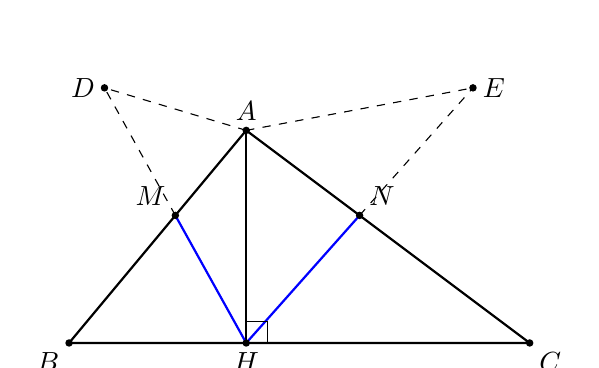
\begin{tikzpicture}[scale=0.9, >=stealth]
  \coordinate (A) at (0,3);
  \coordinate (B) at (-2.5,0);
  \coordinate (C) at (4,0);
  \coordinate (H) at (0,0);
  \coordinate (M) at ($(A)!0.4!(B)$);
  \coordinate (N) at ($(A)!0.4!(C)$);
  \coordinate (D) at ($(M)!-1!(H)$);
  \coordinate (E) at ($(N)!-1!(H)$);
  \draw[thick] (A)--(B)--(C)--cycle;
  \draw[thick] (A)--(H);
  \draw[thick, blue] (H)--(M);
  \draw[thick, blue] (H)--(N);
  \draw[dashed] (M)--(D) (N)--(E);
  \draw[dashed] (A)--(D) (A)--(E);
  \fill (A) circle (1.5pt) node[above] {$A$};
  \fill (B) circle (1.5pt) node[below left] {$B$};
  \fill (C) circle (1.5pt) node[below right] {$C$};
  \fill (H) circle (1.5pt) node[below] {$H$};
  \fill (M) circle (1.5pt) node[above left] {$M$};
  \fill (N) circle (1.5pt) node[above right] {$N$};
  \fill (D) circle (1.5pt) node[left] {$D$};
  \fill (E) circle (1.5pt) node[right] {$E$};
  \draw (0,0.3) -| (0.3,0);
\end{tikzpicture}
\end{center}
\begin{enumerate}[label=\textbf{\alph*)}, leftmargin=0.8cm, itemsep=2pt]
\item (0,25 điểm) Chứng minh tứ giác $AMHN$ là hình chữ nhật.
\item (0,25 điểm) Lấy điểm $D$ sao cho $M$ là trung điểm của $DH$, lấy điểm $E$ sao cho $N$ là trung điểm của $EH$. Chứng minh $AD = AE$.
\item (0,25 điểm) Chứng minh $BC^2 = BD^2 + CE^2 + 2BH \cdot HC$.
\end{enumerate}
\end{ex}
\vspace{0.5mm}

\begin{ex} (0,5 điểm)
Tìm đa thức $P(x)$ biết rằng $P(x)$ chia cho $x - 3$ dư 7; chia cho $x - 2$ dư 5; chia cho $(x - 2)(x - 3)$ được thương là $3x$ và còn dư.
\begin{enumerate}[label=\textbf{\alph*)}, leftmargin=0.8cm, itemsep=2pt]
\item (0,5 điểm) Tìm đa thức $P(x)$.
\end{enumerate}
\end{ex}
\vspace{0.5mm}


\begin{center}
\rule{4cm}{0.4pt}\\
\textit{--- HẾT ---}
\end{center}
\end{document}
